\documentclass[9pt,a4paper]{extarticle}

\usepackage[utf8]{inputenc}
\usepackage[T1]{fontenc}
\usepackage{mathpazo}
\usepackage[scaled=0.92]{helvet}
\usepackage[margin=0.4in,top=0.35in,bottom=0.35in]{geometry}
\usepackage{amsmath,amssymb}
\usepackage{booktabs}
\usepackage{multicol}
\usepackage{enumitem}
\usepackage{setspace}
\usepackage{xcolor}
\usepackage{tikz}
\usetikzlibrary{shapes.gates.logic.US, circuits.logic.US, positioning}

% Spasi yang seimbang (tidak terlalu sesak, tidak terlalu renggang)
\setstretch{1.0}
\setlength{\parindent}{0pt}
\setlength{\parskip}{0.2em}
\setlength{\columnsep}{0.5cm}
\setlength{\columnseprule}{0.3pt}
\setlength{\emergencystretch}{2em}

\setlist[itemize]{leftmargin=1em,noitemsep,topsep=0.5pt,parsep=0pt,itemsep=0.5pt}
\setlist[enumerate]{leftmargin=1.1em,noitemsep,topsep=0.5pt,parsep=0pt,itemsep=0.5pt}
\renewcommand{\arraystretch}{1.15}

% Makro Judul Seksi
\newcommand{\mysect}[1]{%
	\par\vspace{6pt}%
	\noindent{\small\bfseries\sffamily\color{black} #1}\par\vspace{-2pt}%
	\noindent\rule{\linewidth}{0.5pt}\par\vspace{3pt}%
}

% Makro untuk kode inline (JS/Python)
\newcommand{\code}[1]{\colorbox{gray!15}{\texttt{\small #1}}}
\newcommand{\h}[1]{\textbf{#1}}

\pagestyle{empty}

\begin{document}

\begin{center}
	{\Large\bfseries\sffamily Cheat Sheet: Logika Matematika}\\[2pt]
	{\small Matematika Diskrit \textbullet\ TRPL Politeknik Negeri Batam \textbullet\ P6--P7}
\end{center}
\vspace{-6pt}

\begin{multicols}{2}

	\mysect{1. Proposisi \& Gerbang Logika}
	\h{Proposisi:} Pernyataan yang pasti \textbf{True (1)} atau \textbf{False (0)}. Kalimat tanya/perintah, atau variabel bebas ($x>5$) \textbf{bukan} proposisi.

	\vspace{2pt}
	\begin{center}
		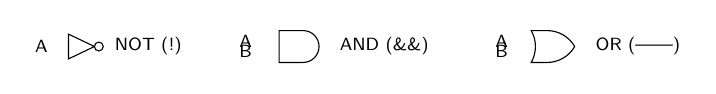
\begin{tikzpicture}[scale=0.8, transform shape, font=\sffamily\footnotesize]
			\node[not gate US, draw, logic gate inputs=nn] (not1) at (0,0) {};
			\node[left=0.2cm of not1] {A};
			\node[right=0.2cm of not1] {NOT (!)};

			\node[and gate US, draw, logic gate inputs=nn] (and1) at (3.5,0) {};
			\node[left=0.3cm of and1.input 1] {A};
			\node[left=0.3cm of and1.input 2] {B};
			\node[right=0.2cm of and1] {AND (\&\&)};

			\node[or gate US, draw, logic gate inputs=nn] (or1) at (7.5,0) {};
			\node[left=0.3cm of or1.input 1] {A};
			\node[left=0.3cm of or1.input 2] {B};
			\node[right=0.2cm of or1] {OR (||)};
		\end{tikzpicture}
	\end{center}
	\vspace{-4pt}

	{\small
		\begin{center}
			\begin{tabular}{@{}c c | c c c c c@{}}
				\toprule
				A & B & AND & OR & XOR & IMPLY & IFF \\
				\midrule
				1 & 1 & 1   & 1  & 0   & 1     & 1   \\
				1 & 0 & 0   & 1  & 1   & 0     & 0   \\
				0 & 1 & 0   & 1  & 1   & 1     & 0   \\
				0 & 0 & 0   & 0  & 0   & 1     & 1   \\
				\bottomrule
			\end{tabular}
		\end{center}}

	\mysect{2. Operator Khusus (Implikasi \& XOR)}
	\h{Implikasi (\(A \to B\)):} "Jika A, maka B".
	\begin{itemize}
		\item \textbf{Vacuously True:} Jika A = 0, hasilnya otomatis \textbf{1} (apa pun nilai B).
		\item \textbf{False mutlak:} Hanya jika A = 1 dan B = 0.
		\item \h{Trik Kode:} \(A \to B \equiv \neg A \lor B\). Di JS: \code{!A || B}.
	\end{itemize}
	\h{XOR (\(\oplus\)):} Benar jika \textbf{TEPAT SATU} bernilai 1. Di JS: \code{A !== B}.

	\mysect{3. Hukum Aljabar Boolean}
	{\small
		\begin{tabular}{@{}l l@{}}
			\toprule
			Hukum           & Rumus                                                      \\
			\midrule
			De Morgan 1     & \(\neg(A \land B) \equiv \neg A \lor \neg B\)              \\
			De Morgan 2     & \(\neg(A \lor B) \equiv \neg A \land \neg B\)              \\
			Negasi Ganda    & \(\neg(\neg A) \equiv A\)                                  \\
			Excluded Middle & \(A \lor \neg A \equiv 1\) (Selalu Benar)                  \\
			Distributif     & \(A \land (B \lor C) \equiv (A \land B) \lor (A \land C)\) \\
			\bottomrule
		\end{tabular}}
	\vspace{2pt}

	\textbf{Penerapan De Morgan di Kode:} \\
	\code{!(A \&\& B)} \(\equiv\) \code{!A || !B} \\
	\code{!(A || B)} \(\equiv\) \code{!A \&\& !B}

	\mysect{4. Penyederhanaan Ekspresi}
	\h{Contoh:} Sederhanakan \(\neg(\neg A \lor B) \lor (A \land B)\).
		{\small
			\begin{enumerate}
				\item \(\equiv (\neg\neg A \land \neg B) \lor (A \land B)\) \textit{(De Morgan)}
				\item \(\equiv (A \land \neg B) \lor (A \land B)\) \textit{(Negasi Ganda)}
				\item \(\equiv A \land (\neg B \lor B)\) \textit{(Distributif)}
				\item \(\equiv A \land 1\) \textit{(Excluded Middle)}
				\item \(\equiv A\) \textit{(Identitas)}
			\end{enumerate}}
	\textit{Kesimpulan:} Kode berantakan \code{if (!(!A || B) || (A \&\& B))} bisa di-*refactor* jadi sekadar \code{if (A)}.

	\mysect{5. Klasifikasi Ekspresi}
	{\small
		\begin{tabular}{@{}l l l@{}}
			\toprule
			Jenis       & Sifat             & Contoh Kode              \\
			\midrule
			Tautologi   & Selalu \textbf{1} & \code{x > 5 || x <= 5}   \\
			Kontradiksi & Selalu \textbf{0} & \code{x > 5 \&\& x <= 5} \\
			Kontingensi & Campuran          & \code{A || B}            \\
			\bottomrule
		\end{tabular}}
	\vspace{2pt}
	\h{Aturan Tabel:} \(n\) variabel $\Rightarrow$ butuh \(2^n\) baris.

	\mysect{6. Studi Kasus: Akses Admin}
	Aturan: Login valid (L), Admin (A), OTP valid (O), DAN akun \textbf{TIDAK} diblokir (B).

	\h{Matematika:} \((L \land A \land O) \land \neg B\) \\
	\h{Kode:} \code{if (L \&\& A \&\& O \&\& !B) \{ ... \}}

	\vspace{2pt}
	\h{Analisis:} Dari 16 kemungkinan ($2^4$), hanya \textbf{1 kondisi} yang True (saat L=1, A=1, O=1, dan B=0). Jika B=1 (diblokir), sehebat apapun loginnya, akses tetap ditolak.

	\mysect{7. Latihan Mandiri (Perpus)}
	Variabel: K (Kartu aktif), T (Tanpa tunggakan), S (Stok buku ada), M (Pinjaman belum maks).

	Aturan: \textbf{K dan T dan S dan M}. \\
	Ekspresi: \(K \land T \land S \land M\) \\
	Kode: \code{if (K \&\& T \&\& S \&\& M) \{ pinjam(); \}}

	\mysect{8. Referensi}
	{\footnotesize Munir (2012); Epp (2010); O'Regan (2023); Slide P6-P7 TRPL Polibatam.}

\end{multicols}

\end{document}
